\section*{Problem 2: Simple Optimization Problem}
\begin{enumerate}
\item
The FOC with respect to $C_0$ reads
\begin{align}
	&-(C_0-\overline C)+\mathbb E[W_0(1+r)-C_0-\overline C]\overset{!}{=}0\\
	\implies&C_0^*=\frac{1}{2}\mathbb E[W_0(1+r)]
	=\frac{W_0}{2}(1+\mathbb E[r]).
\end{align}

\item
The optimal consumption at time 0 only depends on the expected return, irrespective of the variance of $r$. It does not make economic sense since we expect a risk-averse agent would change one's behavior when risk changes.

\item
The FOC with respect to $C_0$ reads
\begin{align}
	&C_0^{-\gamma}-\mathbb E[(W_0(1+r)-C_0)^{-\gamma}]\overset{!}{=}0\\
	\implies&C_0^*=\left(\mathbb E[(W_0(1+r)-C_0)^{-\gamma}]\right)^{-\frac{1}{\gamma}}.
\end{align}

\item
The maximum percentage deviation is 7.8759e-13\%. See Figure \ref{Q2}.
\begin{figure}[htbp]
\begin{center}
	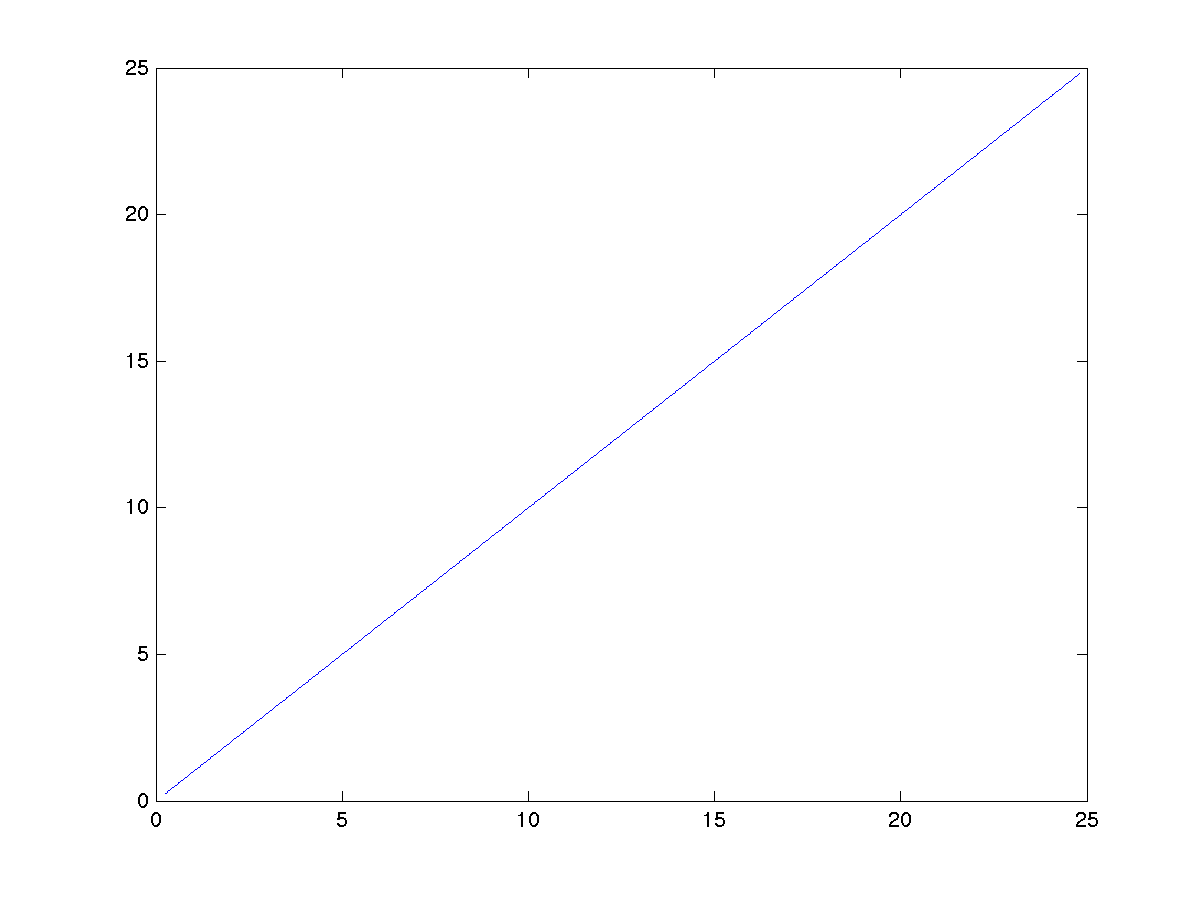
\includegraphics[width=10cm]{Figure/Q2.png}	
\caption{Solution against Chebychev Approximation}
\label{Q2}
\end{center}
\end{figure}

\item
The maximum percentage deviation increases, but not very much.
\end{enumerate}

